%
% Simple template for generating drafts of papers and articles
%
\documentclass[12pt,a4paper]{article}
\usepackage{authblk}
\usepackage{fullpage}
\usepackage{amssymb,amsmath}
\usepackage[utf8x]{inputenc}
\usepackage[T1]{fontenc}
\usepackage{siunitx}
\usepackage[version=3]{mhchem}
\usepackage{isomath}

\usepackage[left]{lineno} % line numbers
\linenumbers

\usepackage{setspace}
\doublespacing

\usepackage[unicode=true]{hyperref}
\hypersetup{breaklinks=true,
            bookmarks=true,
            colorlinks=false,
            pdfborder={0 0 0}}
\urlstyle{same} % don't use a different (monospace) font for urls

\setcounter{secnumdepth}{5}

\usepackage{graphicx}
% \graphicspath{{figures/}}
% % Redefine \includegraphics so that, unless explicit options are
% % given, the image width will not exceed the width or the height of the page.
% % Images get their normal width if they fit onto the page, but
% % are scaled down if they would overflow the margins.
% \makeatletter
% \def\ScaleWidthIfNeeded{%
%  \ifdim\Gin@nat@width>\linewidth
%     \linewidth
%   \else
%     \Gin@nat@width
%   \fi
% }
% \def\ScaleHeightIfNeeded{%
%   \ifdim\Gin@nat@height>0.9\textheight
%     0.9\textheight
%   \else
%     \Gin@nat@width
%   \fi
% }
% \makeatother
% \setkeys{Gin}{width=\ScaleWidthIfNeeded,height=\ScaleHeightIfNeeded,keepaspectratio}%

\usepackage[super, numbers, sort&compress]{natbib}     % or [authoryear]

% Highlighting for review purposes
\usepackage{xcolor}
\usepackage{soul}
\definecolor{reviewyellow}{rgb}{1, 1, 0.6} 
\sethlcolor{reviewyellow}

%%%%%%%%%%%%%%%%%%%%%%%%%%%%%%%%%%%%%%%%%%%%%%%%%%%%%%%%%%%%%%%%%%%%%%%%%%%%%%

% \title{Time-Explicit Life Cycle Optimization: A Framework for Designing Sustainable Transition Pathways}
\title{Time-Explicit Life Cycle Optimization: A Framework for Navigating the Temporal Interdependencies of Sustainable Transition Pathways}
% \title{A Framework for Time-explicit Life Cycle Optimization of Transition Pathways}
\author{Timo Diepers}
\author{Jan Tautorus}
\author{Jan Hartmann}
\author{Niklas von der Assen}
\affil{Institute of Technical Thermodynamics, RWTH Aachen University}

\date{\today}

%%%%%%%%%%%%%%%%%%%%%%%%%%%%%%%%%%%%%%%%%%%%%%%%%%%%%%%%%%%%%%%%%%%%%%%%%%%%%%

\begin{document}

\maketitle

\newpage
\section*{Abstract}
Life cycle optimization (LCO) is a valuable tool for designing sustainable transition pathways, yet current approaches collapse all life cycle stages and emissions to a single point in time, obscuring critical temporal interdependencies. These interdependencies arise from the interplay between \textit{temporal distribution} (life cycle stages occurring at different times) and \textit{temporal evolution} (processes and supply chains changing over time). Distribution determines when exchanges occur, evolution determines their magnitude, and both must be considered jointly to verify whether pathways respect time-specific and dynamically accumulating environmental limits. We present a framework for time-explicit LCO that addresses these two interacting temporal dimensions. We achieve this by extending traditional LCA matrices with an explicit time dimension, using convolution to translate process-relative time lags into absolute system times, while tracking vintage-dependent foreground parameters and linking intermediate flows to time-specific background databases. A case study on integrated methanol and pig iron production reveals capabilities inaccessible to static LCO approaches: strategic overcapacity that accepts stranded fossil assets to accelerate clean technology deployment, vintage-specific dispatch that preferentially utilizes cleaner cohorts, and technology diversification to navigate transient resource bottlenecks. We provide an open-source implementation in the Python package \textit{optimex}, enabling application of time-explicit LCO to design transition pathways that rigorously respect both time-specific and cumulative environmental limits.

\section*{Synopsis}
Processes, emissions, and environmental impacts are fundamentally time-dependent due to their temporal distribution and evolution. This framework captures these interdependencies to design transition pathways respecting both time-dependent and absolute environmental constraints.

\section*{Keywords}
temporal distribution, temporal evolution, transformation pathways, dynamic, prospective life cycle assessment, industrial decarbonization

\section*{\hl{Target Journal: Environmental Science \& Technology}}

\section*{\hl{Reviewer Suggestions}}

\begin{itemize}
    \item \hl{Guillaume Majeau-Bettez --- Polytechnique Montréal, Canada}
    \item \hl{Gonzalo Guillén-Gosálbez --- ETH Zurich, Switzerland}
    \item \hl{Reinout Heijungs --- Vrije Universiteit Amsterdam, The Netherlands}
    \item \hl{Didier Beloin-Saint-Pierre --- EMPA, Switzerland}
    \item \hl{Bhavik Bakshi --- Arizona State University, USA}
    \item \hl{Stefanie Hellweg --- ETH Zurich, Switzerland}
    \item \hl{Sangwon Suh --- Tsinghua University, China}
\end{itemize}

\newpage

\tableofcontents
\newpage

%%%%%%%%%%%%%%%%%%%%%%%%%%%%%%%%%%%%%%%%%%%%%%%%%%%%%%%%%%%%%%%%%%%%%%%%%%%%%%
%%%%%%%%%%%%%%%%%%%%%%%%%%%%%%%%%%%%%%%%%%%%%%%%%%%%%%%%%%%%%%%%%%%%%%%%%%%%%%

\section{Introduction}
Anthropogenic systems must rapidly transform to achieve environmental sustainability \cite{rockstromSafeOperatingSpace2009, steffenPlanetaryBoundariesGuiding2015}. Environmental sustainability encompasses two fundamental sets of constraints: absolute limits—such as finite mineral stocks \cite{GlobalCriticalMinerals2025} and cumulative carbon budgets \cite{intergovernmentalpanelonclimatechangeipccClimateChange20212023b, rogeljEstimatingTrackingRemaining2019}—and time-specific limits, dictating maximum rates at which resources can be extracted or emissions assimilated by the biosphere \cite{GlobalCriticalMinerals2025, thomassenPlanetaryBoundaryMineral2024}. Successful transitions towards sustainability must rigorously account for both sets of constraints to prevent systemic overshoot and ensure feasibility.

While Integrated Assessment Models (IAMs) are primary instruments for navigating these transitions, they typically rely on highly aggregated representations of technological systems\cite{weyantContributionsIntegratedAssessment2017}. Without technological granularity, IAMs cannot identify the specific supply chain bottlenecks or emission profiles that trigger a violation of time-specific limits \cite{pauliukIndustrialEcologyIntegrated2017}. While sector- or process-specific optimization models improve on the technological resolution, they often neglect indirect and non-greenhouse gas emissions, risking environmental burden shifting\cite{fodstadNextFrontiersEnergy2022, reinertSecMODOpenSourceModular2022}.

To include indirect emissions and consider a broader range of environmental impacts besides climate change, optimization models have been increasingly coupled with Life Cycle Assessment (LCA) in so-called Life Cycle Optimization (LCO)\cite{pieragostiniProcessOptimizationConsidering2012a, blancoLifeCycleAssessment2020, reinertSecMODOpenSourceModular2022, ferdousIntegrationLCATEA2023a, azapagicLinearProgrammingTool1998, katelhonStochasticTechnologyChoice2016, lechtenbergPULPOFrameworkEfficient2024}. However, current LCO approaches typically rely on a static representation of life cycle impacts. By assuming all processes and emissions across life cycles occur simultaneously, static LCO effectively collapses the temporal dimension. This simplification makes it impossible to verify if a pathway respects time-specific limits, as the model cannot distinguish between an emission or resource consumption occurring today or a decade from now. 

The issue of time-differentiation has been increasingly addressed by the LCA community \cite{beloin-saint-pierreAddressingTemporalConsiderations2020,lueddeckensTemporalIssuesLife2020,sohnDefiningTemporallyDynamic2020,suAssessmentModelsDynamic2021,lang-quantzendorffTimedifferentiatingMethodsLife2025}, differentiating two interacting temporal dimensions: \textit{temporal distribution} and \textit{temporal evolution} \cite{mullerTimeexplicitLifeCycle2025}. First, real-world life cycles can span multiple years or decades, leading to time lags between different life cycle stages and their associated emissions and resource consumption (\textit{temporal distribution}) \cite{collingeDynamicLifeCycle2013,beloin-saint-pierreESPAEnhancedStructural2014,tiruta-barnaFrameworkComputationalTool2016,cardelliniTemporalisGenericMethod2018}. Second, processes and supply chains change over time, leading to differing emissions and resource consumption profiles at different points in time (\textit{temporal evolution}). This is particularly relevant for systems undergoing rapid transformation, such as the energy sector, where electricity mixes and manufacturing supply chains are rapidly decarbonizing \cite{zimmermannProspectiveTimeresolvedLCA2015, mendozabeltranWhenBackgroundMatters2020, sacchiPRospectiveEnvironMentalImpact2022}.

In transition pathway design, these two temporal dimensions are inextricably linked. The \textit{distribution} of processes determines when an environmental exchange occurs, while the \textit{evolution} of the production system determines the magnitude of that exchange at that specific moment. Consequently, both dimensions simultaneously dictate whether a transition pathway stays within time-specific limits (by shifting the timing and scale of annual peaks) and absolute limits (by altering the total cumulative inventory over the entire transition period). To ensure that pathways are truly sustainable, optimization models must account for these temporal interdependencies.

While the \textit{assessment} of transition pathways under consideration of temporal distribution and evolution is enabled by time-explicit LCA\cite{mullerTimeexplicitLifeCycle2025}, its integration into optimization frameworks for the \textit{design} of transition pathways remains incomplete. Current attempts solely focus on the aspect of temporal evolution: \citet{reinertEnvironmentalImpactsFuture2021} couple an energy system model with prospective LCA, and \citet{thakkerMappingPathNetzero2024} optimize a transition of the chemical industry incorporating learning curves and ongoing decarbonization. Similarly, \citet{hungECOPT2AdaptableLife2022} consider the temporal evolution of the electricity sector, alongside stock dynamics. Still, these contributions disregard the temporal distribution of life cycles, assuming life cycle exchanges occur at the moment of a technology's installation. This creates a structural inability to model the interaction between system-specific time lags and supply chain shifts. For example, ignoring the decades-long lag between a facility’s construction and its end-of-life means the model cannot account for the fact that decommissioning will occur in a fundamentally different—and likely less carbon-intensive—background system. Consequently, such models risk misdetermining the total cumulative impacts and may generate transition pathways that appear to respect absolute limits while violating time-specific limits during periods of intensive infrastructure buildup. As two recent review conclude, full time-differentiation remains a significant gap in LCO \cite{lang-quantzendorffTimedifferentiatingMethodsLife2025,turnerSystematicReviewLife2025}.

In this work, we propose a framework for time-explicit LCO of transition pathways. By simultaneously considering the temporal distribution and evolution of processes and their environmental exchanges, our framework enables the identification of pathways that rigorously respect both time-dependent and absolute environmental constraints. The framework is flexible and broadly applicable across sectors, offering a robust foundation for designing sustainable transformation pathways. An implementation of the framework is provided in the open-source Python package \textit{optimex}, seamlessly integrating with the \textit{Brightway} LCA framework \cite{mutelBrightwayOpenSource2017} and the \textit{pyomo} optimization framework \cite{bynumPyomoOptimizationModeling2021}. The application of time-explicit LCO is demonstrated in a case study on an integrated industrial system co-producing methanol and pig iron.

%%%%%%%%%%%%%%%%%%%%%%%%%%%%%%%%%%%%%%%%%%%%%%%%%%%%%%%%%%%%%%%%%%%%%%%%%%%%%%
%%%%%%%%%%%%%%%%%%%%%%%%%%%%%%%%%%%%%%%%%%%%%%%%%%%%%%%%%%%%%%%%%%%%%%%%%%%%%%

\section{Time-Explicit Life Cycle Optimization Framework}

As the basis for time-explicit LCO, we first review the mathematical formulation of static LCO in Section \ref{sec:static_lco}. Building on this, we then introduce a mathematical framework for time-explicit LCO in Section \ref{sec:math_framework}, extending static LCO to simultaneously consider temporal distribution and evolution of life cycle processes and their environmental exchanges. Next, in Section \ref{sec:operationalization}, we outline the operationalization of the proposed framework, detailing how the mathematical framework can be integrated in common LCA and LCO modeling practices. Finally, Section \ref{sec:implementation} briefly introduces a Python-based implementation of the framework in the \textit{optimex} package.
%%%%%%%%%%%%%%%%%%%%%%%%%%%%%%%%%%%%%%%%%%%%%%%%%%%%%%%%%%%%%%%%%%%%%%%%%%%%%%

\subsection{Foundation} \label{sec:static_lco}

In traditional matrix-based LCA, environmental impacts $\vectorsym{h}$ are calculated by characterizing a life cycle inventory $\vectorsym{g}$ using a characterization matrix $\matrixsym{Q}$:
\begin{equation}\label{eq:lca_h}
\vectorsym{h} = \matrixsym{Q} \, \vectorsym{g}
\end{equation}

The life cycle inventory $\vectorsym{g}$ is typically determined from the intervention matrix $\matrixsym{B}$ and a scaling vector $\vectorsym{s}$:
\begin{equation}\label{eq:lca_g}
\vectorsym{g} = \matrixsym{B} \, \vectorsym{s}
\end{equation}

In turn, $\vectorsym{s}$ is determined from the following relationship between the technology matrix $\matrixsym{A}$ and the functional unit or demand vector $\vectorsym{f}$ as follows:
\begin{equation}\label{eq:lca_s}
\vectorsym{s} = \matrixsym{A}^{-1} \, \vectorsym{f}
\end{equation}

In LCO, the technology matrix $\matrixsym{A}$ is not square, as multiple processes (i.e., columns) can produce the same products (i.e., rows). This makes $\matrixsym{A}$ non-invertible, so $\vectorsym{s}$ can not be determined from Eq. \ref{eq:lca_s}. Instead, the scaling vector $\vectorsym{s}$ is made the decision variable of an optimization problem, where $\vectorsym{s}$ is determined such that the demand $\vectorsym{f}$ is satisfied while minimizing or maximizing some objective function. A linear LCO problem with the objective to minimize environmental impact $h^{\mathrm{c}}$, where $c$ is a specific chosen impact category, can be formulated as:
\begin{subequations}\label{eq:static_lco}
\begin{align}
\min_{\vectorsym{s}} \quad & h^{\mathrm{c}} = \matrixsym{Q}^{\mathrm{c}} \, \vectorsym{g} = \matrixsym{Q}^{\mathrm{c}} \, \matrixsym{B} \, \vectorsym{s} \label{eq:static_lco:a}\\
\text{s.t. } & \matrixsym{A} \, \vectorsym{s} = \vectorsym{f}, \label{eq:static_lco:b}\\
& \vectorsym{s} \ge \vectorsym{0}. \label{eq:static_lco:c}
\end{align}
\end{subequations}

%%%%%%%%%%%%%%%%%%%%%%%%%%%%%%%%%%%%%%%%%%%%%%%%%%%%%%%%%%%%%%%%%%%%%%%%%%%%%%

\subsection{Formulation} \label{sec:math_framework}

In the static LCO formulation described in Eq. \ref{eq:static_lco}, neither temporal distribution nor temporal evolution of processes and emissions can be considered. In this Section, we extend this formulation to a time-explicit LCO in five steps: (1) introducing an explicit temporal dimension in all matrices and vectors, (2) considering time lags in the supply chain through convolution, (3) distinguishing foreground and background systems, (4) incorporating temporal evolution through vintage-dependent foreground parameters and scenario-specific background databases, and (5) differentiating installation- and operation-dependent flows. Finally, we compose the fully time-explicit LCO problem.

\subsubsection{Time-Indexed Matrices and Vectors}

To allow for the LCA matrices and tensors to reflect time-specific quantities, we add time as an explicit dependency to all matrices and vectors from Eq. \ref{eq:static_lco}, as originally proposed for dynamic LCA by \citet{collingeDynamicLifeCycle2013}. The environmental impact in a specific category $h^{\mathrm{c}}$ is determined by summing over all time steps $t \in \mathcal{T}$:
\begin{equation}\label{eq:dyn_g}
h^{\mathrm{c}} = \sum_{t \in \mathcal{T}} \matrixsym{Q}^{\mathrm{c}}_t \, \vectorsym{g}_t =  \sum_{t \in \mathcal{T}} \matrixsym{Q}^{\mathrm{c}}_t \, \matrixsym{B}_t \, \vectorsym{s}_t
\end{equation}
with:
\begin{equation}\label{eq:dyn_A}
  \matrixsym{A}_t \, \vectorsym{s}_t =  \vectorsym{f}_t \quad \forall t \in \mathcal{T}  
\end{equation}

This formulations enables consideration of different production systems, emissions, and characterization factors (i.e., dynamic Life Cycle Impact Assessmentm, LCIA), for different points in time. However, each time-slice is evaluated separately here. That means that a process at time $t_i$ still can only supply products to other processes at $t_i$, but not to processes at another time $t_{i+1}$, though this would be desirable to reflect the time lags that inevitably exist in real-world production systems. 

\subsubsection{Reflecting Time Lags through Convolution}
To enable time-explicit LCO to reflect time lags, we add a differentiation between two different time parameters. System time $t$ corresponds to absolute points in time with respect to the entire system. Process time $\delta$ represents a relative time delta with respect to a defined installation time of a certain process. Using this process time, we can model  time-relative in- or outputs from or to the technosphere ($\matrixsym{A}$) and the biosphere ($\matrixsym{B}$). The scaling vector $\vectorsym{s}$ and the demand vector $\vectorsym{f}$ still refer to absolute points in time. This way, $\vectorsym{s}$ can reflect a process happening at a specific absolute point in time $t$, e.g., January 1, 2025, but exchanges of that process, such as its end-of-life treatment, to happen $\delta=10$ years later, which would translate to January 1, 2035. To mathematically reflect this translation of time deltas to absolute points in time, we use convolution, such that:
\begin{subequations}\label{eq:convolution}
\begin{align}
& (\matrixsym{A}*\vectorsym{s})_t = \sum_{\delta \in \Delta_t} \matrixsym{A}_{\delta}\,\vectorsym{s}_{t-\delta}, \\
& (\matrixsym{B}*\vectorsym{s})_t = \sum_{\delta \in \Delta_t} \matrixsym{B}_{\delta}\,\vectorsym{s}_{t-\delta}.
\end{align}
\end{subequations}

where $\Delta_t$ is the subset of valid time deltas at system time $t$, such that $\Delta_t = \{ \delta \in \Delta \mid t - \delta \in \mathcal{T} \}$, and $\Delta$ denotes the set of all process time deltas for which exchanges are defined.

The time-explicit inventory $\vectorsym{g}_t$ can thus be determined from:
\begin{equation}
    \vectorsym{g}_t = (\matrixsym{B}*\vectorsym{s})_t
\end{equation}

and solving:
\begin{equation}
    (\matrixsym{A}*\vectorsym{s})_t =  \vectorsym{f}_t
\end{equation}

\subsubsection{Distinguishing Foreground and Background Systems}

A common modeling convention in LCA is to differentiate between a foreground system, i.e., a specific system under study, and a background system, representing the broader economy and supply chains, typically sourced from LCI databases. To enable this distinction in time-explicit LCO and allowing for the subsequent consideration of temporal evolution in foreground and background systems, we divide the technosphere into a foreground system $\matrixsym{A}^{\text{fg}}$ and a background system $\matrixsym{A}^{\text{bg}}$. Similarly, we split the corresponding biosphere matrices into $\matrixsym{B}^{\text{fg}}$ and $\matrixsym{B}^{\text{bg}}$. From these, we can obtain separate life cycle inventory vectors $\vectorsym{g}^{\mathrm{fg}}$ and $\vectorsym{g}^{\mathrm{bg}}$ for the foreground and background, respectively.

The foreground system inventory results from convolving the foreground biosphere matrix with the scaling vector:
\begin{equation}\label{eq:g_fg}
\vectorsym{g}^{\mathrm{fg}}_t = \left(\matrixsym{B}^{\mathrm{fg}} * \vectorsym{s}\right)_t
\end{equation}

For the background system inventory, we first calculate how much of each background process is demanded based on the foreground's intermediate flows to the background:
\begin{equation}\label{eq:f_bg}
    \vectorsym{f}_t^{\mathrm{bg}} = \left(\matrixsym{A}^{\mathrm{fg}} * \vectorsym{s} \right)_t
\end{equation}

The aggregated elementary flows of a unitary production from a background process can be expressed through what \citet{heijungsComputationalStructureLife2002} call the intensity matrix $\matrixsym{\Lambda}$:
\begin{equation}\label{eq:lambda}
    \matrixsym{\Lambda} = \matrixsym{B}^{\mathrm{bg}} \, \left(\matrixsym{A}^{\mathrm{bg}}\right)^{-1}
\end{equation}

The background inventory $\vectorsym{g}^{\mathrm{bg}}$ then results from:
\begin{equation}\label{eq:g_bg}
\vectorsym{g}^{\mathrm{bg}}_t = \matrixsym{\Lambda} \, \vectorsym{f}^{\mathrm{bg}}_t
\end{equation}

The environmental impact $h^{\mathrm{c}}_t$ can then be calculated from:
\begin{equation}\label{eq:b_fg_bg}
h^{\mathrm{c}}_t = \matrixsym{Q}^{\mathrm{c}}_t \, \left( \vectorsym{g}^{\mathrm{fg}}_t + \vectorsym{g}^{\mathrm{bg}}_t \right)
\end{equation}

\paragraph{Foreground Evolution: Vintage-Dependent Parameters}

To reflect technological improvement of the foreground system in the foreground inventory (Eq.~\ref{eq:g_fg}), we extend the foreground matrices to depend on the vintage (installation year) of each process unit. We introduce the vintage $v \in \mathcal{T}$ as an additional index. For a process installed at time $v$ and operating at process time $\delta$, the technosphere and biosphere coefficients become $a^{\text{fg}}_{p,i,\delta,v}$ and $b^{\text{fg}}_{p,e,\delta,v}$, respectively. The convolution from Eq.~\ref{eq:convolution} generalizes to:

\begin{subequations}\label{eq:convolution_vintage}
\begin{align}
& \left(\matrixsym{A}^{\text{fg}}*\vectorsym{s}\right)_t = \sum_{v \in \mathcal{V}_t} \matrixsym{A}^{\text{fg}}_{\delta=t-v,\, v}\,\vectorsym{s}_{v}, \\
& \left(\matrixsym{B}^{\text{fg}}*\vectorsym{s}\right)_t = \sum_{v \in \mathcal{V}_t} \matrixsym{B}^{\text{fg}}_{\delta=t-v,\, v}\,\vectorsym{s}_{v}.
\end{align}
\end{subequations}

Here, $\mathcal{V}_t = \{v \in \mathcal{T} \mid t - v \in \Delta\}$ is the set of vintages with exchanges occurring at system time $t$, determined by whether the process time $\delta = t - v$ falls within the defined time deltas $\Delta$. For example, a process installed at $v = 2025$ evaluated at $t = 2030$ has $\delta = 5$, meaning it is five years into its life cycle. The coefficient $a^{\text{fg}}_{p,i,\delta,v}$ thus captures both the life cycle stage (via $\delta = t-v$) and technological generation (via $v$).

To express foreground technology evolution, we apply multiplicative scaling factors $\phi_{p,i,v}$ to base coefficients:

\begin{equation}\label{eq:evolution_scaling}
    a^{\text{fg}}_{p,i,\delta,v} = \phi_{p,i,v} \cdot a^{\text{fg,base}}_{p,i,\delta},\quad
    b^{\text{fg}}_{p,e,\delta,v} = \phi_{p,e,v} \cdot b^{\text{fg,base}}_{p,e,\delta}
\end{equation}

where $a^{\text{fg,base}}_{p,i,\delta}$ and $b^{\text{fg,base}}_{p,e,\delta}$ are the base (vintage-independent) coefficients. A scaling factor $\phi_{p,i,v} = 0.7$ indicates a 30\% improvement relative to the base amount of the respective exchange.

\paragraph{Background Evolution: Time-Specific Scenario Databases}

In addution to the specific improvements of foreground processes, the background system is also subject to temporal evolution. To reflect this, we allow demands from the background system (Eq.~\ref{eq:f_bg}) to be fulfilled from different time-specific background databases $b \in \mathcal{B}$, depending on the time $t$ at which this demand occurs. The mapping from times $t$ to databases $b$ is handled by a mapping matrix $\matrixsym{M}$. In the simplest case, $\matrixsym{M}$ is an identity matrix, corresponding to a one-to-one mapping of time $t$ to corresponding timestamps of the background databases. However, in the case that the background databases are only available for fewer discrete time steps than $t$, e.g., only reflect 5-year-steps, $\matrixsym{M}$ can also be constructed such that it interpolates between database times, distributing a demand across time with certain weights. The background inventory from Eq.~\ref{eq:g_bg} then generalizes to:
\begin{equation}\label{eq:g_bg_temporal}
\vectorsym{g}^{\mathrm{bg}}_t = \left( \sum_{b \in \mathcal{B}} \matrixsym{\Lambda}_b \, \matrixsym{M}_{b,t} \right) \vectorsym{f}^{\mathrm{bg}}_t
\end{equation}


\subsubsection{Differentiating Installation- and Operation-Dependent Flows}

In traditional LCA and LCO, processes are implicitly assumed to always be operated at a fixed capacity, as all process exchanges are temporally aggregated. In reality, the operation levels of processes can vary over time. As time-explicit LCO captures the temporal distributino of life cycles, it enables considering flexible process operation with respect to a certain amount of installed capacity. To achieve this, we split the decision variable of the optimization problem in two components: capacity installation $\vectorsym{s}_v$ (indexed by vintage $v$) and operational level $\vectorsym{o}_{t,v}$ (indexed by system time $t$ and vintage $v$). 

By introducing the vintage-specific operational variable $\vectorsym{o}_{t,v}$, the model can explicitly distinguish between the activities of different cohorts of the same technology fleet. This enables a vintage-specific dispatch (merit order), where the cleanest available vintages are utilized first at any given time $t$.

To differentiate between installation and operation, we colect all operation-depdentent flows in a set $\mathcal{O}$. We then define separate technosphere and biosphere matrices for operation ($\matrixsym{A}^{\mathrm{op}}$ and $\matrixsym{B}^{\mathrm{op}}$) and capacity installations ($\matrixsym{A}^{\mathrm{cap}}$ and $\matrixsym{B}^{\mathrm{cap}}$). The operation matrices $\matrixsym{A}^{\mathrm{op}}_{v}$ and $\matrixsym{B}^{\mathrm{op}}_{v}$ contain the per-unit-operation coefficients for flows marked as operation-dependent, with vintage-specific values reflecting technology evolution (Eq.~\ref{eq:evolution_scaling}).

For the capacity matrices $\matrixsym{A}^{\mathrm{cap}}_{\delta, v}$ and $\matrixsym{B}^{\mathrm{cap}}_{\delta, v}$, we isolate flows occurring outside the operational phase (e.g., construction and end-of-life):
\begin{subequations}\label{eq:cap_op_split}
\begin{align}
a^{\text{cap}}_{p,i,\delta,v} &=
  \begin{cases}
    a^\text{fg}_{p,i,\delta,v} & \text{if } i \notin \mathcal{O}\\
    0 & \text{otherwise}
  \end{cases}, \quad
b^{\text{cap}}_{p,e,\delta,v} =
  \begin{cases}
    b^\text{fg}_{p,e,\delta,v} & \text{if } e \notin \mathcal{O} \\
    0 & \text{otherwise}
  \end{cases}
\end{align}
\end{subequations}

The foreground inventory contribution at time $t$ now sums over all active vintage cohorts. For each process $p$, the set of operable vintages is $\mathcal{V}^{\mathrm{op}}_{t} = \{v \in \mathcal{T} \mid v \leq t \text{ and } t-v \leq L_p\}$, where $L_p$ is the process-specific lifetime. Note that $\mathcal{V}^{\mathrm{op}}_{t} \subseteq \mathcal{V}_t$, as operable vintages must also have exchanges defined at that time. The foreground inventory becomes:
\begin{equation}\label{eq:g_fg_flex}
    \vectorsym{g}^{\mathrm{fg,flex}}_t = \sum_{v \in \mathcal{V}_t} \matrixsym{B}^{\mathrm{cap}}_{\delta=t-v,\, v}\,\vectorsym{s}_{v} + \sum_{v \in \mathcal{V}^{\mathrm{op}}_t} \matrixsym{B}^{\mathrm{op}}_{v} \, \vectorsym{o}_{t,v}
\end{equation}

The total demand $\vectorsym{f}_t$ is satisfied by the sum of production across all operable vintages, while each vintage's dispatch is constrained by its individual deployed capacity $\vectorsym{s}_v$:
\begin{subequations}
\begin{align}
    & \sum_{v \in \mathcal{V}^{\mathrm{op}}_t} \matrixsym{A}^{\mathrm{op}}_{v} \, \vectorsym{o}_{t,v} \geq \vectorsym{f}_{t} \\
    & \vectorsym{o}_{t,v} \leq \vectorsym{s}_{v} \quad \forall v \in \mathcal{V}^{\mathrm{op}}_t
\end{align}
\end{subequations}

Finally, the background inventory in Eq.~\ref{eq:g_bg_temporal} is reformulated to reflect this disaggregated demand:
\begin{equation}\label{eq:g_bg_flex}
    \vectorsym{g}^{\mathrm{bg,flex}}_t = \sum_{b \in \mathcal{B}} \matrixsym{\Lambda}_b \, \matrixsym{M}_{b,t} \Big[ \sum_{v \in \mathcal{V}_t} \matrixsym{A}^{\mathrm{cap}}_{\delta=t-v,\, v}\,\vectorsym{s}_{v} + \sum_{v \in \mathcal{V}^{\mathrm{op}}_t} \matrixsym{A}^{\mathrm{op}}_{v} \, \vectorsym{o}_{t,v} \Big]
\end{equation}

\subsubsection{Complete Optimization Problem Formulation}

The final optimization problem for time-explicit LCO is:
\begin{subequations}\label{eq:final_opt_problem}
\begin{align}
\min_{\vectorsym{s}_{v},\, \vectorsym{o}_{t,v}} \quad
& \sum_{t \in \mathcal{T}}
\matrixsym{Q}^{\mathrm{c}}_{t}
\left( \vectorsym{g}^{\mathrm{fg,flex}}_t + \vectorsym{g}^{\mathrm{bg,flex}}_t \right)\\
\text{s.t.} \quad 
& \vectorsym{o}_{t,v} \leq \vectorsym{s}_{v} 
\quad \forall t \in \mathcal{T}, v \in \mathcal{V}^{\mathrm{op}}_t, \label{eq:opt_op:b} \\
& \sum_{v \in \mathcal{V}^{\mathrm{op}}_t} \matrixsym{A}^{\mathrm{op}}_{v} \, \vectorsym{o}_{t,v} \geq \vectorsym{f}_{t} 
\quad \forall t \in \mathcal{T},\label{eq:opt_op:c} \\
& \vectorsym{s}_{v} \geq \vectorsym{0} \quad \forall v \in \mathcal{T}, \quad \vectorsym{o}_{t,v} \geq \vectorsym{0} 
\quad \forall t \in \mathcal{T}, v \in \mathcal{V}^{\mathrm{op}}_t.
\end{align}
\end{subequations}

%%%%%%%%%%%%%%%%%%%%%%%%%%%%%%%%%%%%%%%%%%%%%%%%%%%%%%%%%%%%%%%%%%%%%%%%%%%%%%

\subsection{Operationalization} \label{sec:operationalization}

In the following, we describe the operationalization of the proposed mathematical framework for time-explicit LCO. Figure \ref{fig:method_overview} summarizes the main steps. First, we explain how foreground systems are modeled and processed, including the temporal information, vintage-specific evolution, and the differentiation of installation- and operation-dependent flows (Section \ref{sec:operationalization:temporalization}). Next, we detail how time-specific values are inserted into time-explicit matrices (Section \ref{sec:operationalization:tensor_construction}). Finally, we outline the formulation of the optimization problem (Section \ref{sec:operationalization:opt_formulation}).

\begin{figure}[!ht]
    \centering
    \noindent
    \includegraphics[width=0.45\textwidth]{figs/method_overview.pdf} 
    \caption{Time-explicit LCO workflow.}
    \label{fig:method_overview}
\end{figure}

\subsubsection{Preparing the Foreground System} \label{sec:operationalization:temporalization}
The first step of a time-explicit LCO is to prepare the foreground system including the set of possible processes to install and operate. To allow for flexible modeling of multiple processes sharing a product or single processes with multiple outputs, we treat processes and products as separate entities in the foreground. Consequently, processes are not tied to a single reference product, and the optimization algorithm can choose between competing production routes. Conversely, for the background system, the choice of modeling structure is invariant, as it contains no decision variables and production routes are fixed.

Next, temporal information is embedded in the product system model, reflecting the temporal distributions of intermediate and elementary flows. To achieve this, we follow the approach introduced by \citet{beloin-saint-pierreESPAEnhancedStructural2014} and later used by \citet{cardelliniTemporalisGenericMethod2018} (dynamic LCA) and \citet{mullerTimeexplicitLifeCycle2025} (time-explicit LCA). The idea is to specify temporal information on the process-level via process-relative temporal distributions (rTDs). These rTDs define what share of the exchanged amount happens at what time, with respect to the consuming process (or emitting process for elementary flows). RTDs therefore consist of two arrays, one for the time(-deltas), and one for the amount shares. Here, we use the implementation by \citet{cardelliniTemporalisGenericMethod2018}, which allows to directly save rTDs as additional metadata to the flows in LCI databases. The underlying temporal resolution of rTDs is completely flexible, and can range from hourly to yearly values.

To reflect time lags between processes, we use convolution (cf. Eq. \ref{eq:convolution}) of the rTDs between the timing of process installation (as indicated through $\vectorsym{s}_v$) and the exchanges defined in $\matrixsym{A}_{\delta}$. This way, if a process capacity is installed in the year 2030, construction processes can be modeled to happen at $\delta = (-2)$ years before that, translating to 2028. Operational inputs could uniformly be spread from $\delta=0$ until $\delta=10$, so from 2030 until 2040, with end-of-life treatment scheduled at $\delta=11$, translating to 2041. Through more complex rTD definitions, also temporal dynamics in further upstream processes can be approximated, which is further discussed in Section \ref{sec:discussion}.

In addition to the temporal information, we further need to mark flows that are operation-dependent, so  they can be scaled separate from capacity installation. This classification can be added as metadata through a boolean flag for each flow.

To reflect the temporal evolution of foreground processes through vintage-dependent parameters (cf. Eq.~\ref{eq:evolution_scaling}), technology evolution can be specified as additional metadata for intermediate and elementary flows, providing time-specific scaling factors for exchange values.

\subsubsection{Constructing Time-explicit Matrices} \label{sec:operationalization:tensor_construction}
Depending on the timing of intermediate and elementary flows, the underlying production systems, exchanged amounts and characterization factors can change. 

For the foreground system, time-specific values for intermediate and elementary flows can be directly derived from the defined rTDs. These are inserted into the respective technosphere and biosphere matrices $\matrixsym{A}_{\delta}$ and $\matrixsym{B}_{\delta}$, which are both already set up to reflect time deltas rather than absolute points in time (cf. Eq. \ref{eq:convolution}). The previously entered boolean flag for operation-dependent flows then decides whether the values are inserted in the operation variants ($\matrixsym{A}^{\mathrm{op}}_{v}$, $\matrixsym{B}^{\mathrm{op}}_{v}$) or the capacity variants ($\matrixsym{A}^{\mathrm{cap}}_{\delta, v}$, $\matrixsym{B}^{\mathrm{cap}}_{\delta, v}$) of the matrices. Additionally, the time-specific scaling factors for technology evolution defined in Section \ref{sec:operationalization:temporalization} are applied to the corresponding exchange values.

To reflect the temporal evolution of background production systems, we use time-specific background databases representing the state of the production system at single absolute points in time. Such databases can be created based on own assumptions or external scenarios, e.g., using tools like premise\cite{sacchiPRospectiveEnvironMentalImpact2022}. The representative time of a database needs to be defined by the user as database metadata. The temporal resolution of the provided background databases is flexible and is not required to be the same as the temporal resolution of the rTDs, as time resolutions are bridged by the mapping matrix $M$. 

Finally, time-specific values for the characterization matrices $\matrixsym{Q}_t$ can be specified. The proposed method is agnostic with respect to the source of these values. For example, time-specific characterization factors can be derived from dynamic LCIA methods, e.g., absolute metrics such Radiative Forcing (RF), Absolute Global Warming Potential (AGWP) or Absolute Global Temperature Change Potential (AGTP), relative (i.e., normalized with respect to $\ce{CO2}$) metrics like dynamic Global Warming Potential (GWP$_{\mathrm{dyn}}$) \cite{levasseurConsideringTimeLCA2010}, or even prospective-dynamic metrics such as the recently proposed prospective AGWP (pAGWP) and prospective AGTP (pAGTP) \cite{barbosawatanabeProspectiveCharacterizationFactors2026}.

\subsubsection{Defining Objectives and Constraints} \label{sec:operationalization:opt_formulation}
As the basis for the optimization problem formulation, an impact category must be defined as the objective that is to be minimized. Next, a time-specific demand can be defined, specifying product quantities and the points in time at which they are required. This demand can be expressed as an rTD with respect to a user-defined (absolute) reference time. Together with the time-explicit LCA matrices introduced above, these inputs parameterize the optimization model in Eq. \ref{eq:final_opt_problem}. Optionally, further constraints can be added to the optimization problem, such as existing (brownfield) process capacities or eithertime-dependent or cumulative limits on process installations, environmental impact categories or individual intermediate or elementary flows. 


%%%%%%%%%%%%%%%%%%%%%%%%%%%%%%%%%%%%%%%%%%%%%%%%%%%%%%%%%%%%%%%%%%%%%%%%%%%%%%

\subsection{Implementation} \label{sec:implementation}

The proposed time-explicit LCO framework is implemented in the open-source Python package \textit{optimex} \cite{Optimex2025}. For its LCA-related capabilities, \textit{optimex} builds on the open-source LCA framework \textit{Brightway}\cite{mutelBrightwayOpenSource2017}. For dynamic LCIA, \textit{optimex} can directly source methods from the \textit{Brightway} library dynamic\_characterization\cite{Dynamic_characterization2025}. For all optimization-related operations, \textit{optimex} uses the open-source optimization framework \textit{pyomo}\cite{bynumPyomoOptimizationModeling2021}. Additional information and instructions are available in \textit{optimex}’ comprehensive online documentation \cite{OptimexDocumentationTimeexplicit2025}.

%%%%%%%%%%%%%%%%%%%%%%%%%%%%%%%%%%%%%%%%%%%%%%%%%%%%%%%%%%%%%%%%%%%%%%%%%%%%%%
%%%%%%%%%%%%%%%%%%%%%%%%%%%%%%%%%%%%%%%%%%%%%%%%%%%%%%%%%%%%%%%%%%%%%%%%%%%%%%

%%%%%%%%%%%%%%%%%%%%%%%%%%%%%%%%%%%%%%%%%%%%%%%%%%%%%%%%%%%%%%%%%%%%%%%%%%%%%%

\section{Application}

To demonstrate the capabilities of time-explicit LCO, we apply the proposed framework to an integrated industrial system co-producing methanol and pig iron through a combination of conventional and decarbonized pathways. The general purpose of this case study is to illustrate the capabilities of time-explicit LCO, focusing on methodological implications rather than providing a comprehensive assessment of methanol and pig iron production systems. The production system and optimization setup are described in Section \ref{sec:case_study_setup}. The case study results are presented in Section \ref{sec:results}. The full case study code is available as an annotated Jupyter Notebook in the \textit{optimex} GitHub repository \cite{Optimex2025}.

\subsection{Case Study Setup} \label{sec:case_study_setup}

The considered production system for methanol and pig iron is illustrated in Fig. \ref{fig:production_system_overview}. 

\begin{figure}[!ht]
    \centering
    \noindent
    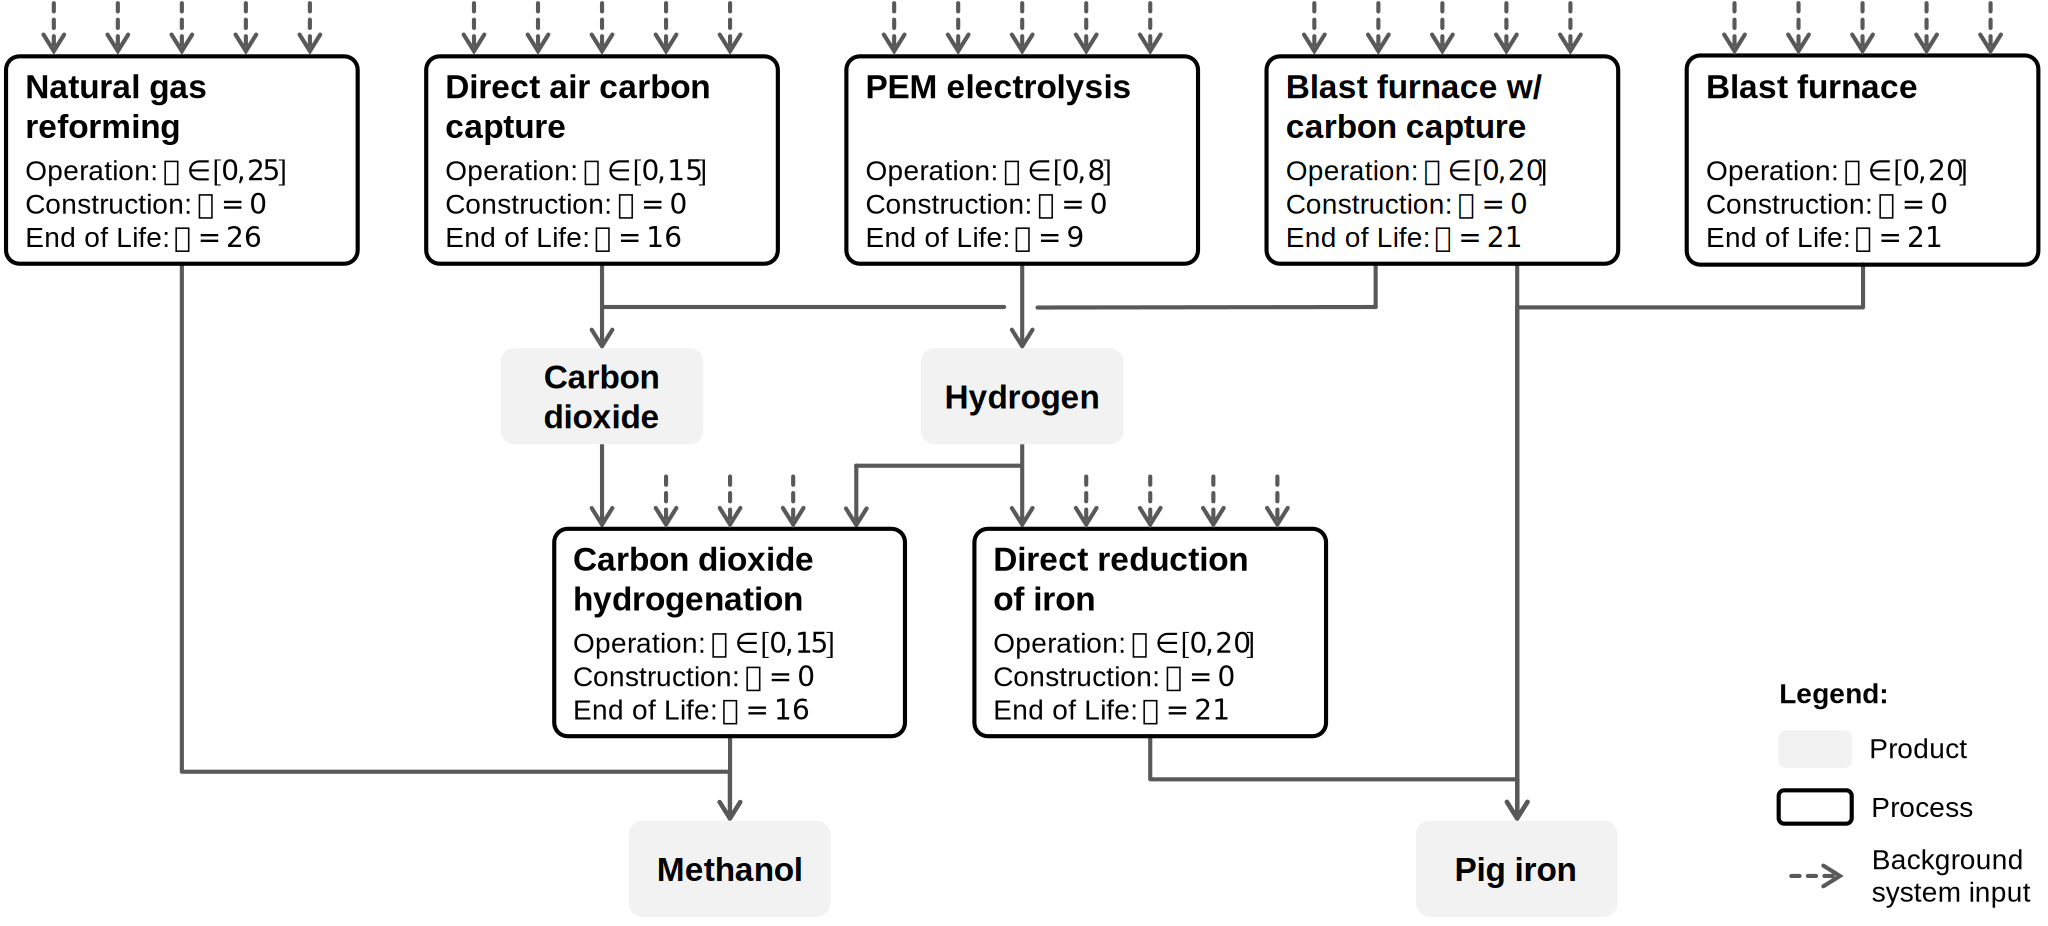
\includegraphics[width=\textwidth]{figs/product_system.pdf} 
    \caption{Production system for methanol and pig iron.}
    \label{fig:production_system_overview}
\end{figure}

The production system is designed to meet a constant annual demand of 1~Mt for both methanol and pig iron from 2025 to 2050. This is modeled as a brownfield optimization problem, accounting for existing fossil-based production infrastructure. We assume that 0.5~Mt of yearly capacity was installed in both 2005 and 2015 for both methanol (via natural gas reforming) and pig iron (via standard blast furnace), totaling 1~Mt of legacy capacity at the start of the transition period. 

From the beginning of the transition period, the system is presented with additional process and supply chain choices to satisfy the demands. For methanol synthesis, the model can choose between conventional natural gas reforming (lifetime $L=25$ years) and $\ce{CO2}$ hydrogenation ($L=15$ years). The latter offers flexible $\ce{CO2}$ sourcing, either from point-source capture via a Blast Furnace with Carbon Capture (BF-CC) or from atmospheric removal via Direct Air Carbon Capture (DAC). Similarly, pig iron production is diversified through standard blast furnaces, BF-CC, and Hydrogen-based Direct Reduction of Iron (H$_2$-DRI). Notably, these production routes are highly intertwined: the BF-CC process co-produces pig iron and the $\ce{CO2}$ feedstock for methanol synthesis, while Proton Exchange Membrane (PEM) electrolysis ($L=8$ years) provides the hydrogen required for both $\ce{CO2}$ hydrogenation and the H$_2$-DRI route. Each process is associated with specific installation- and operation-dependent intermediate and elementary flows, distributed across distinct time-relative phases: construction ($\delta \leq 0$), operation ($\delta \in [0, L]$), and end-of-life treatment ($\delta > L$). Process-specific inventories are derived from the ecoinvent 3.12 database \cite{wernetEcoinventDatabaseVersion2016}.

The optimization objective is the minimization of climate impacts, which we assess through the cumulative RF with a fixed end year for the consideration of all emissions set to 2125. The cumulative RF corresponds to the total energy commitment to the atmosphere caused by the inventory. For further analysis of climate impacts, we additionally assess the underlying instantaneous RF, representing the actual warming rate caused by the inventory at each point in time. As an additional impact category, we consider the water use impact, which we assess through static characterization factors from Environmental Footprint 3.1 \cite{jointresearchcentreeuropeancommissionUpdatedCharacterisationNormalisation2023}

To demonstrate the framework's versatility, we define three modeling scenarios. The "Baseline" scenario has no temporal evolution, i.e., foreground parameters and background supply chains are fixed at 2025 states. The "Evolution" scenario assumes continuous improvement across the system. In the foreground, efficiency gains are modeled through vintage-dependent scaling factors, including decreasing electricity consumption for PEM electrolysis, decreasing electricity and heat consumption for DAC, and decreasing electricity consumption and reduced direct fugitive $\ce{CO2}$ emissions for the $\ce{CO2}$ hydrogenation process. Simultaneously, the background system undergoes extensive decarbonization. We utilize a set of prospective ecoinvent 3.12 databases derived from the REMIND-EU Shared Socioeconomic Pathway 2 (SSP2) PkBudg1000 scenario (projecting below 2°C warming by 2100), covering the period from 2020 to 2100 and created via \textit{premise}\cite{sacchiPRospectiveEnvironMentalImpact2022}. Finally, the "Constrained Evolution" scenario introduces resource bottlenecks on top of the Evolution scenario, including an annual limit to the impact on water use ($3 \cdot 10^5$ $\text{m}^3$-eq) and a cumulative limit on Iridium extraction (0.125 kg limit) as a proxy for critical mineral scarcity. 

All further modeling details and assumptions are available in an annotated Jupyter Notebook in the \textit{optimex} GitHub repository \cite{Optimex2025}.

\subsection{Results} \label{sec:results}
Figure \ref{fig:results} summarizes the time-explicit LCO results for the integrated methanol and pig iron production system across scenarios. 

\begin{figure}[!h]
    \centering
    \noindent
    \includegraphics[width=\textwidth]{figs/results_and_impacts.pdf} 
    % \caption{Installation, operation and environmental impacts of the optimized methanol and pig iron production system over the transition pathway.}
    \label{fig:results}
\end{figure}

In the Baseline scenario (Fig.~\ref{fig:results} a-1 to g-1), the model identifies no incentive for technological change, maintaining fossil-based natural gas reforming and blast furnaces through 2050. The installed capacity (dashed lines) exactly matches the demand, representing 100\% utilization of installed capacity. Once installed capacities reach the end of their lifetime, new capacities are immediately installed to replace them. Considering the climate impact, the annual cumulative RF (e-1) declines over time. This is a methodological consequence of the fixed 2125 time horizon: later emissions are integrated over a shorter remaining duration, effectively "cutting off" their long-term impact. In contrast, the instantaneous RF curves (f-1) depict the actual warming rate caused by the inventory. While these curves rise, their slope flattens over time. This is driven by the atmospheric decay of greenhouse gases: as the inventory accumulates, the radiative forcing lost to the decay of past emissions increasingly counteracts the forcing added by new emissions, causing the net growth rate to slow. For water use, the impact remains constant throughout the period (g-1) because we use static characterization factors.

In the Evolution scenario (Fig.~\ref{fig:results} a-2 to g-2), the model identifies a phased transition toward electrification starting in 2033. As background electricity impacts decrease, the system switches to $\ce{CO2}$ hydrogenation for methanol and H$_2$-DRI for pig iron. A significant observation is the emergence of overcapacities (dashed lines exceeding solid bars). The model finds that an earlier switch to electrification routes, and the resulting savings in operational emissions, outweighs the impacts of "wasted" fossil-based brownfield capacities. Consequently, fossil capacities are idled as the cleaner technology cohorts take over. Figures~\ref{fig:results} (e-2) and (f-2) highlight the interplay between technology improvement and climate trajectories. For instance, for electrolysis, even when production levels remain constant after 2033 (d-2), the yearly cumulative RF bars decline due to the decarbonization of background inputs and efficiency improvements, and more drastically than the decline due to the decreasing time horizon for integration, as shown in (e-1). Accordingly, the slope of the corresponding instantaneous RF curves (f-2) also decreases more with cleaner production vintages being dispatched over time.

Finally, the Constrained Evolution scenario (Fig.~\ref{fig:results} a-3 to g-3) demonstrates the framework's ability to navigate resource bottlenecks. The previous evolution scenario revealed that hydrogen-based routes carry substantial water impacts (g-2). By imposing annual water availability caps and a cumulative limit on Iridium for PEM stacks, the model is forced to diversify its technological portfolio. The system shifts back toward a mix of technologies in later years, utilizing BF-CC for iron production to stay within resource limits, but slightly raising climate impacts.

Overall, these results illustrate that time-explicit LCO identifies transition pathways that navigate complex temporal interdependencies, which remain hidden in static assessments. By resolving transient resource peaks (Fig.~\ref{fig:results} g) and accounting for the shifting climate impacts of technologies (Fig.~\ref{fig:results} e, f), the framework enables the design of feasible pathways that respect both time-specific resource bottlenecks and cumulative environmental limits.

%%%%%%%%%%%%%%%%%%%%%%%%%%%%%%%%%%%%%%%%%%%%%%%%%%%%%%%%%%%%%%%%%%%%%%%%%%%%%%

%%%%%%%%%%%%%%%%%%%%%%%%%%%%%%%%%%%%%%%%%%%%%%%%%%%%%%%%%%%%%%%%%%%%%%%%%%%%%%
%%%%%%%%%%%%%%%%%%%%%%%%%%%%%%%%%%%%%%%%%%%%%%%%%%%%%%%%%%%%%%%%%%%%%%%%%%%%%%

\newpage
\section{Discussion} \label{sec:discussion}

Designing transition pathways that respect real-world environmental constraints requires optimization models capable of capturing when emissions occur, not just their aggregated magnitudes. The time-explicit LCO framework presented in this work addresses this requirement by jointly modeling the temporal distribution of life cycle stages and the temporal evolution of production systems. Where existing LCO approaches either neglect time entirely or only account for prospective changes in background systems, our framework tracks the full temporal profile of both intermediate and elementary exchanges---from construction through operation to end-of-life---while simultaneously reflecting technological progress and supply chain decarbonization. Mathematically, this is achieved by expanding traditional LCA matrices with a temporal dimension, indexing the technosphere and biosphere matrices by process time deltas and vintage ($\matrixsym{A}_{\delta,v}$, $\matrixsym{B}_{\delta,v}$) and enabling interaction between time slices through convolution (Eq.~\ref{eq:convolution}).

The case study (Section~\ref{sec:results}) demonstrates how this interplay between installation timing, operational emissions, and technological evolution leads to transition pathways that differ substantially from static approaches. Several unique capabilities emerge: the identification of non-obvious trade-offs, such as strategic overcapacities where early investment in cleaner technologies offsets embodied infrastructure impacts, vintage-specific merit order dispatch that preferentially utilizes cleaner technology cohorts, and the ability to navigate transient resource bottlenecks by diversifying technology portfolios. These capabilities depend not only on temporal resolution in the inventory but also on the choice of impact assessment method. The framework supports both static and dynamic characterization, with the latter necessary for capturing time-sensitive impacts. For climate change, dynamic metrics such as RF are essential when considering the different atmospheric lifetimes of greenhouse gases and their time-dependent energy absorptions. The framework extends to other impact categories where timing matters, such as water use.

Time-explicit LCO is broadly relevant across sectors where temporal dynamics are decisive, for example: (1) systems depending on evolving upstream processes, where inputs such as electricity, steel, or hydrogen undergo rapid decarbonization; (2) early-stage technologies with improving efficiencies, where vintage-dependent performance gains are significant; (3) circular economy planning with long material residence times, where decades-long lags between installation and end-of-life create temporal mismatches between primary demand and secondary supply; (4) time-resolved carbon accounting, such as biogenic feedstocks with varying rotation periods, temporary carbon storage in $\ce{CO2}$-based products, or carbon dioxide removal technologies with varying temporal profile of $\ce{CO2}$ removals; and (5) multi-regional supply chains with divergent evolution, where sourcing decisions must account for heterogeneous decarbonization trajectories across production regions alongside region-specific total availabilities.

To lower the barrier to application of time-explicit LCO, we provide an open-source implementation in the Python package \textit{optimex} \cite{Optimex2025}, building on the \textit{Brightway} LCA framework \cite{mutelBrightwayOpenSource2017} and the \textit{pyomo} optimization framework \cite{bynumPyomoOptimizationModeling2021}. Users can leverage familiar LCA modeling approaches to define production systems, and then extend them with rTDs, vintage-dependent evolution factors, and the classification of installation and operation-dependent flows, enabling independent scaling of infrastructure required for vintage-specific process operation. By facilitating the integration of time-specific databases from \textit{premise}\cite{sacchiPRospectiveEnvironMentalImpact2022} and dynamic characterization functions from \textit{dynamic\_characterization}\cite{Dynamic_characterization2025}, \textit{optimex} automatically constructs the optimization model from these inputs, allowing practitioners to focus on process and system modeling.

\subsection{Limitations}

Unlike dynamic LCA approaches that propagate temporal distributions through entire multi-tier supply chains \cite{beloin-saint-pierreESPAEnhancedStructural2014,tiruta-barnaFrameworkComputationalTool2016,cardelliniTemporalisGenericMethod2018}, we apply convolution only at a single tier. To illustrate: when deploying a PEM electrolyzer in 2030, convolution can distribute its direct exchanges across time: construction inputs at $\delta=-1$ (2029), operational inputs from $\delta=0$ to $\delta=8$ (2030--2038), and end-of-life flows at $\delta=9$ (2039). However, temporal information is not propagated further upstream: our approach treats upstream supply chains as temporally aggregated at the time of the direct exchange. Previous work has shown that this simplification can meaningfully affect results, particularly for products with long supply chains or significant upstream contributions \cite{pinsonnaultTemporalDifferentiationBackground2014}.

This single-tier limitation reflects a fundamental incompatibility between recursive supply chain graph traversal and linear optimization. Setting up an optimization problem requires fixed parameters that define how decision variables relate to constraints and objectives. With multi-tier convolution, these parameters would encode the temporal profile of all upstream emissions. However, those upstream timings depend on when the consuming process is installed, which shifts the entire upstream cascade accordingly. Since installation timing is the decision variable being optimized, the coefficients cannot be determined until the problem is solved, yet the problem cannot be solved without knowing the parameters first. In standard dynamic LCA, installation time is known upfront, allowing complete graph traversal. In optimization, this circular dependency prevents the same approach. Multi-tier convolution could theoretically be approximated by pre-computing temporal profiles for all possible installation times, but this would dramatically increase problem size. Alternatively, iterative schemes could alternate between optimization and updating upstream profiles, though at the cost of global optimality guarantees.

Two practical workarounds exist where finer upstream temporal resolution is needed. First, critical processes can be moved into the foreground system, allowing rTDs to be explicitly specified on their exchanges. Second, supply chain time lags can be approximated by pre-computing time-resolved emission profiles using dynamic LCA and mapping them as rTDs on corresponding elementary flows---though this does not capture supply chain evolution when the upstream process itself is temporally distributed.

In addition to this methodological limitation, time-explicit LCO also inherits the data challenges of time-explicit LCA \cite{mullerTimeexplicitLifeCycle2025}. Data on (1) the temporal distribution of processes, (2) the temporal evolution of product systems, and (3) time-specific characterization methods is scarce. While tools like \textit{premise} \cite{sacchiPRospectiveEnvironMentalImpact2022} have improved access to time-specific LCI data, open datasets on temporal process profiles and dynamic characterization methods remain limited. Our implementation addresses this by defaulting to static data when temporal information is unavailable, allowing analyses to proceed with partial temporal coverage.

\subsection{Extensions and Future Directions}

The ability to resolve exact emission timing has implications beyond environmentally sustainable transition planning. In economic carbon markets, emissions are typically priced using static metrics like GWP100, irrespective of when they occur. Yet as carbon prices are projected to rise toward 2050, the economic cost of emissions becomes time-dependent. Time-explicit LCO could integrate such price trajectories directly, enabling optimization that minimizes financial risk alongside environmental impact. This is particularly relevant for sectors with long-lived infrastructure, where decisions to delay construction or prioritize early operational savings yield vastly different economic outcomes.

The framework also provides a foundation for modeling circular economy dynamics. Internal material circularity in the foreground system can already be represented: secondary materials from end-of-life activities of earlier vintages enter product balances at specific system times, becoming available for subsequent installation phases. This, for example, enables pathways that optimize recycling loops within primary resource extraction limits. Such internal modeling could be complemented by interfacing with dynamic material flow analysis \cite{kullmannCombiningWorldsEnergy2021}, allowing stocks and flows external to the system boundary to be accounted for and providing more comprehensive constraints on resource availability \cite{gaoDynamicMaterialFlow2018, hungECOPT2AdaptableLife2022}.

Finally, by formulating time-explicit LCO as a mathematical optimization problem, the framework opens access to a broad range of established optimization methods. Future work can leverage multi-objective optimization to reveal trade-offs, or near-optimal methods to identify diverse pathways that align with political feasibility. Additionally, stochastic programming can ensure robustness against uncertainty, while mixed-integer and non-linear formulations capture discrete investments and economies of scale, collectively refining time-explicit LCO as a tool for strategic planning of sustainable transitions.

\newpage\clearpage

\renewcommand\refname{References}
\bibliographystyle{unsrtnat}
\bibliography{optimex}
\newpage

\end{document}

%%%%%%%%%%%%%%%%%%%%%%%%%%%%%%%%%%%%%%%%%%%%%%%%%%%%%%%%%%%%%%%%%%%%%%%%%%%%%%